\chapter{Конструкторский раздел}

\section{Функциональная модель оптимизации метода сжатия страниц}

Разрабатываемая оптимизация метода сжатия страниц памяти с использованием подсчета информационной энтропии состоит из следующих этапов:

\begin{enumerate}
	\item Вычисление значения информационной энтропии с помощью метода подсчета.
	\item Сравнение вычисленного значения информационной энтропии с пороговым значением.
	\item Сжатие страницы в случае, если полученное значение информационной энтропии меньше порогового значения.
\end{enumerate}

IDEF0-диаграмма первого уровня, формализующая основные этапы оптимизации сжатия страниц оперативной памяти, приведена на рисунке \ref{img:first-level}.
    
\includeimage
    {first-level}
    {f}
    {h}
    {1.0\textwidth}
    {IDEF0-диаграмма первого уровня}

\section{Требования к разрабатываемому программному обеспечению}

Согласно описанию этапов решения поставленной задачи разрабатываемое программное обеспечение должно:

\begin{itemize}
	\item вычислять информационную энтропию страницы оперативной памяти, которая является вектором $a = (a_1\text{ }a_2\text{ }\dotso\text{ }a_N)$ размером $N$, равным размеру страницы памяти, $0 \leq a_i \leq 255$;
	\item если вычисленное значение меньше порогового, сжимать входную страницу память, то есть, получать вектор $b = (b_1\text{ }b_2\text{ }\dotso\text{ }b_M)$ размером $M \neq N$, $0 \leq b_i \leq 255$;
	\item если вычисленное значение больше или равно пороговому, входная страница памяти не должна изменяться.
\end{itemize}

\section{Структура разрабатываемого программного обеспечения}

Структура загружаемого модуля ядра zram включает в себя следующие части:
\begin{itemize}
	\item модуль блочного устройства, который выполняет функции создания, настройки и удаления дисков, обработки операций записи и чтения страниц и получения статистики;
	\item модуль сжатия, который выполняет функции сжатия и восстановления данных, а также настройку этих операций.
\end{itemize}

Функция сжатия данных, предоставляемая модулем сжатия, вызывается в модуле блочного устройства во время обработки записи страницы на диск, как представлено на рисунке \ref{img:zram-structure}.

\includeimage
    {zram-structure}
    {f}
    {h}
    {0.6\textwidth}
    {Структура модуля zram}

Согласно выделенным к разрабатываемому программному обеспечению требованиям сжатие страницы должно проводиться только в случае, если полученное значение информационной энтропии меньше порогового. Поэтому для выполнения поставленной задачи необходимо изменить функцию записи страницы на диск модуля блочного устройства. Структура разрабатываемого программного обеспечения показана на рисунке \ref{img:structure}.

\begin{figure}[H]
	\begin{center}
		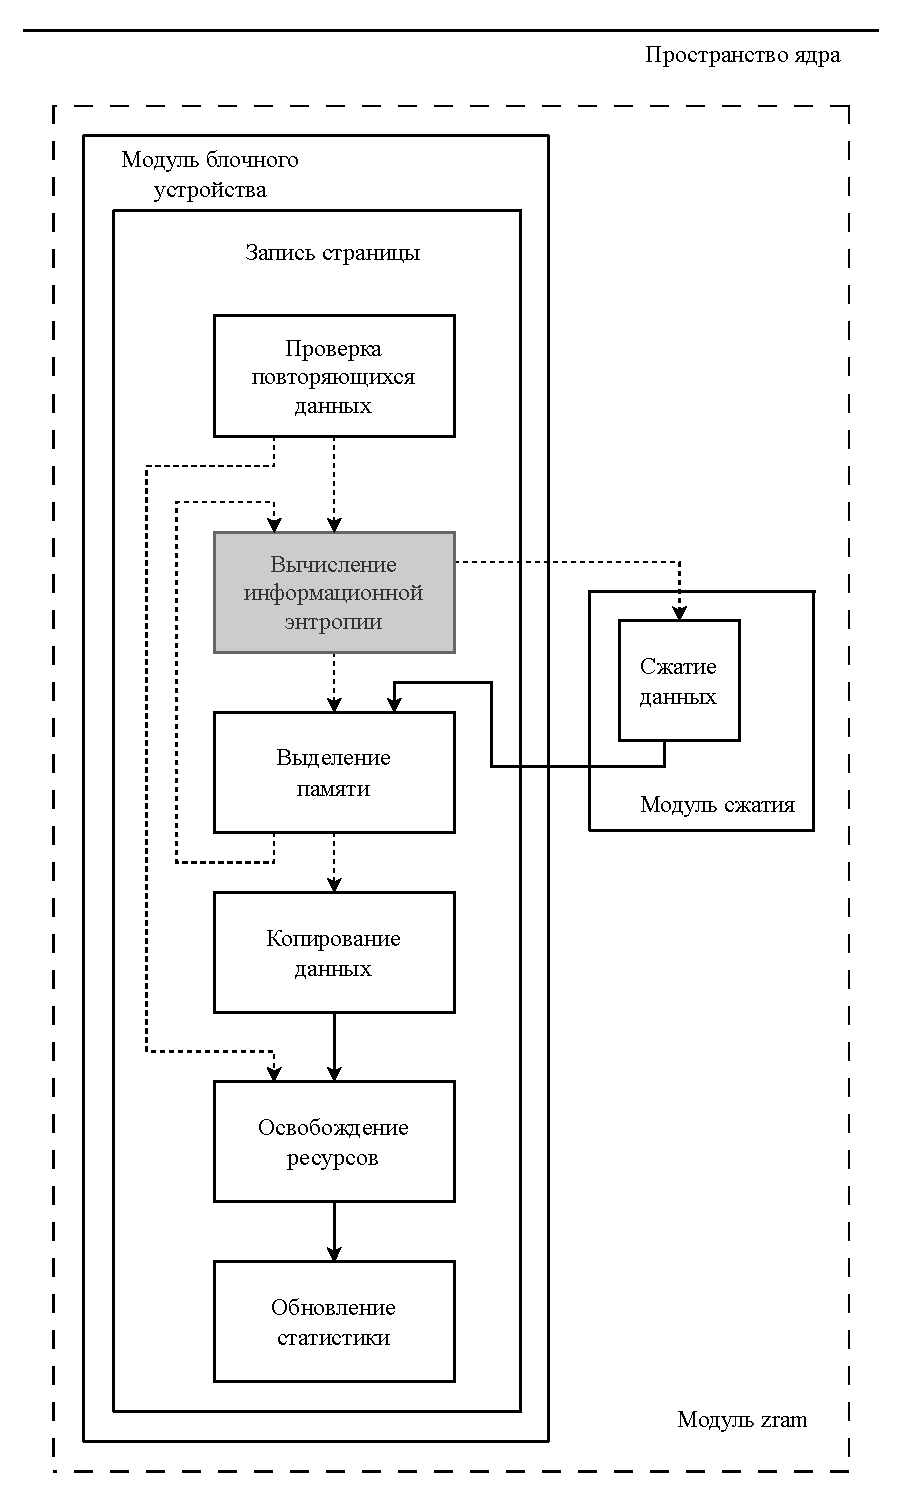
\includegraphics[scale=0.6]{inc/img/structure.pdf}
	\end{center}
	\captionsetup{justification=centering}
	\caption{Структура разрабатываемого программного обеспечения}
	\label{img:structure}
\end{figure}

\section{Схемы алгоритмов}

На рисунке \ref{img:get-sw-entropy} приведена схема алгоритма подсчета информационной энтропии методом скользящего окна.

\begin{figure}[H]
	\begin{center}
		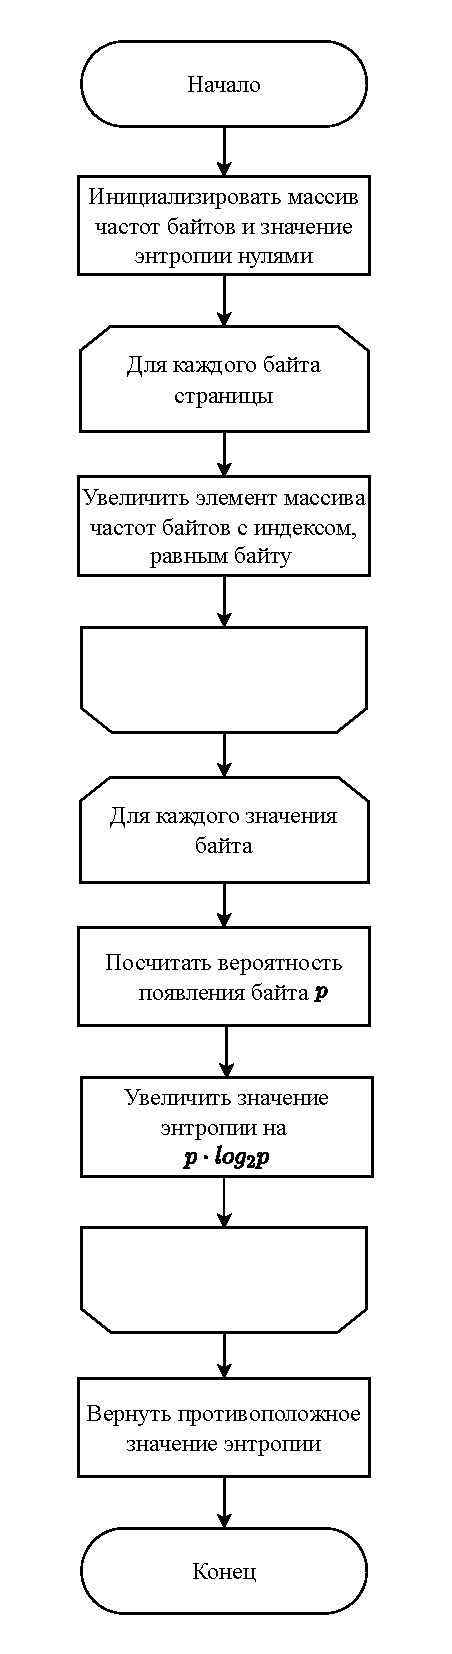
\includegraphics[scale=0.75]{inc/img/get-sw-entropy.pdf}
	\end{center}
	\captionsetup{justification=centering}
	\caption{Схема алгоритма метода скользящего окна}
	\label{img:get-sw-entropy}
\end{figure}

На рисунке  приведена схема алгоритма подсчета информационной энтропии биномиальным методом.

На рисунке  представлена схема алгоритма сжатия страницы.

\section{Выбор типов и структур данных}

Входными и выходными данными является страница памяти, которая задается вектором размером меньшим или равным размеру страницы в байтах, состоящим из значений от нуля до 255. Поэтому для представления страницы в методе подсчета информационной энтропии должен использоваться массив типа unsigned char размером, равным размеру страницы в байтах.

При выполнении операций с числами с плавающей точкой в режиме пользователя ядро перехватывает системное прерывание и переходит из режима вычислений с целыми числами в режим с плавающей точкой. Если использовать режим с плавающей точке в пространстве ядра, необходимо сохранять и восстанавливать состояние регистров с плавающей точкой математического сопроцессора. Вычисления с числами с плавающей точкой в режиме ядра выполнять не рекомендуется. Поэтому для представления числовых величин должен использоваться целочисленный тип данных. 

\section{Тестирование}

\section*{Вывод}

В данном разделе были разработаны основные этапы оптимизации метода сжатия страниц памяти с использованием подсчета информационной энтропии. Были сформулированы требования к разрабатываемому программному решению. Взаимодействие компонетов системы было представлено в виде структуры. Кроме того были представлены схемы алгоритмов подсчета информационной энтропии и сжатия страниц памяти модулем блочного устройства загружаемого модуля zram. Было обосновано использование типов и структур данных.
